\documentclass[hidelinks,aspectratio=169]{beamer}
\usepackage[italian]{babel} 
\usepackage[utf8]{inputenc} 
\usepackage{fourier} 

%Slide colors
\usetheme{Madrid}
%\usecolortheme{beaver}

% Images
\usepackage{graphicx}
\usepackage{caption}
\usepackage{subcaption}
\usepackage{float}
\graphicspath{{Immagini}}

% Stop hyphenation
\usepackage[none]{hyphenat}

% Minipages in the same line
\usepackage{tabularx}

% Coloring links
\usepackage{xcolor}

% Enumerate abc
\usepackage{enumerate}

% Redefines caption setup in way to remove "Figure:"
\usepackage{caption}
\captionsetup[figure]{labelformat=empty}

% To set element positions
\usepackage{ragged2e}

% To insert the logo in the bottom right conrner
\usepackage{tikz}

% License
\usepackage[
type={CC},
modifier={by-nc-sa},
version={4.0},
]{doclicense}

%------------------- Commands zone --------------------

%Command to zoom in
\usepackage{mwe}
\makeatletter
\newsavebox\zb@x
\newcounter{z@@m}
\usepackage{calc}
\newdimen\B@r\newdimen\P@r
\newdimen\@zw\newdimen\@zh\newdimen\@zd

\newcommand{\zoombox}[2][0]{%
	\leavevmode%
	\sbox\zb@x{#2}%
	\setlength\B@r{1pt*\ratio{\wd\zb@x}{\ht\zb@x+\dp\zb@x}}%
	\setlength\P@r{1pt*\ratio{\paperwidth}{\paperheight}}%
	\ifdim\B@r>\P@r\relax%
	\setlength\@zw{\wd\zb@x}\setlength\@zh{\@zw*\ratio{\paperheight}{\paperwidth}}%
	\setlength\@zd{(\@zh-\ht\zb@x-\dp\zb@x)*\real{0.5}+\dp\zb@x}%
	\setlength\@zh{\@zh-\@zd}%
	\else%
	\setlength\@zh{\ht\zb@x+\dp\zb@x}%
	\setlength\@zw{\@zh*\ratio{\paperwidth}{\paperheight}}%
	\setlength\@zh{\ht\zb@x}\setlength\@zd{\dp\zb@x}%
	\fi%
	\makebox[0pt][l]{\makebox[\wd\zb@x][c]{\makebox[\@zw][l]{%
				\pdfdest name {zbfs\thez@@m} fitr
				width  \@zw\space
				height \@zh\space
				depth  \@zd\space
	}}}%
	\pdfdest name {zb\thez@@m} fitr
	width  \wd\zb@x\space
	height \ht\zb@x\space
	depth  \dp\zb@x\space
	\immediate\pdfannot 
	width  \wd\zb@x\space
	height \ht\zb@x\space
	depth  \dp\zb@x\space
	{%
		/Subtype/Link/H/N
		/Border [0 0 #1 [1 2]]
		/A <<
		/S/JavaScript
		/JS (
		if(typeof(zoomed)=='undefined'||!zoomed){
			var lastView=this.viewState;
			if(app.fs.isFullScreen) this.gotoNamedDest('zbfs\thez@@m');
			else this.gotoNamedDest('zb\thez@@m');
			zoomed=true;
		}else{
			this.viewState=lastView;
			zoomed=false;
		}
		)
		>>
	}%
	\usebox{\zb@x}%
	\stepcounter{z@@m}%
} 
\makeatother

%------------------- Header --------------------
\title[]{\textbf{Think in 3-D} \\ \vspace*{3mm} \small \textbf{Tecnologie 3-D per riparazioni e sostituzioni di componentistica}}
\author[Think in 3-D]{}
\date{}
\logo{\includegraphics[scale=0.04]{logo_bianco.png}}

\begin{document}
	
	\begin{frame}[plain]
		\maketitle
			\vspace*{5mm}
			\begin{tabularx}{\linewidth}{XX}
				{
				\begin{center}
					\vspace*{-20mm}
					\zoombox{\includegraphics[scale=0.2]{logo_bianco.png}}
				\end{center}
				}&{
				\begin{center}
					\vspace*{-11mm}
						\large
						\textbf{Francesco Rombaldoni}\newline\newline
						\href{f.rombaldoni@campus.uniurb.it}{\textcolor{blue}{f.rombaldoni@campus.uniurb.it}}
				\end{center}
			}
			\end{tabularx}
	\end{frame}	
	%------------------- Fine prima slide --------------------
	
	%------------------- Seconda slide --------------------
	\begin{frame}{\textbf{Il problema}}
		\begin{tabularx}{\linewidth}{XX}
			{
				\vspace*{20mm}
				\begin{itemize}
					\item Ho subito bisogno di un pezzo di ricambio. \newline \newline \textbf{\textcolor{red}{Qualcuno mi aiuti!}}
				\end{itemize}
			}&{
				\begin{center}
					\zoombox{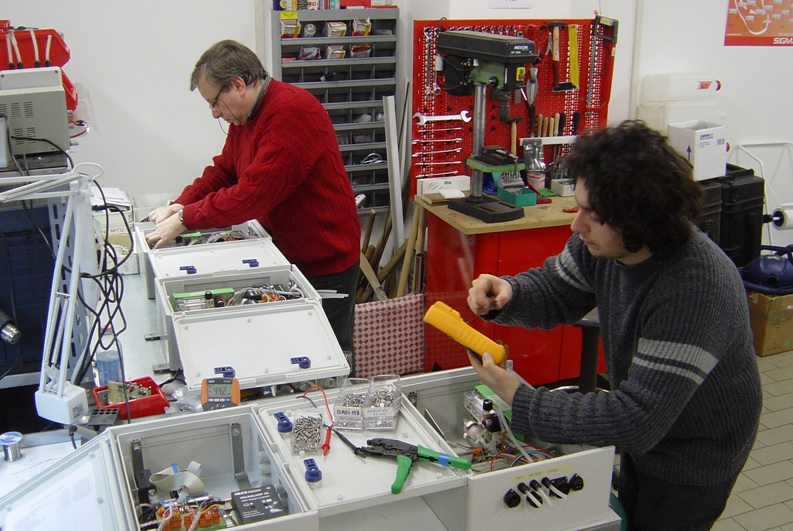
\includegraphics[scale=0.35]{Page1.png}}
				\end{center}
			}
		\end{tabularx}
	\end{frame}
	
	%------------------- Terza slide --------------------
	\begin{frame}{\textbf{La soluzione}}
		\begin{itemize}
			\item L'unione tra i moderni programmi di modellazione 3-D e le nuove tecnologie per la stampa in 3-D permette di risolvere economicamente ed efficacemente il problema.
		\end{itemize}
		\vspace*{5mm}
		\begin{center}
			\zoombox{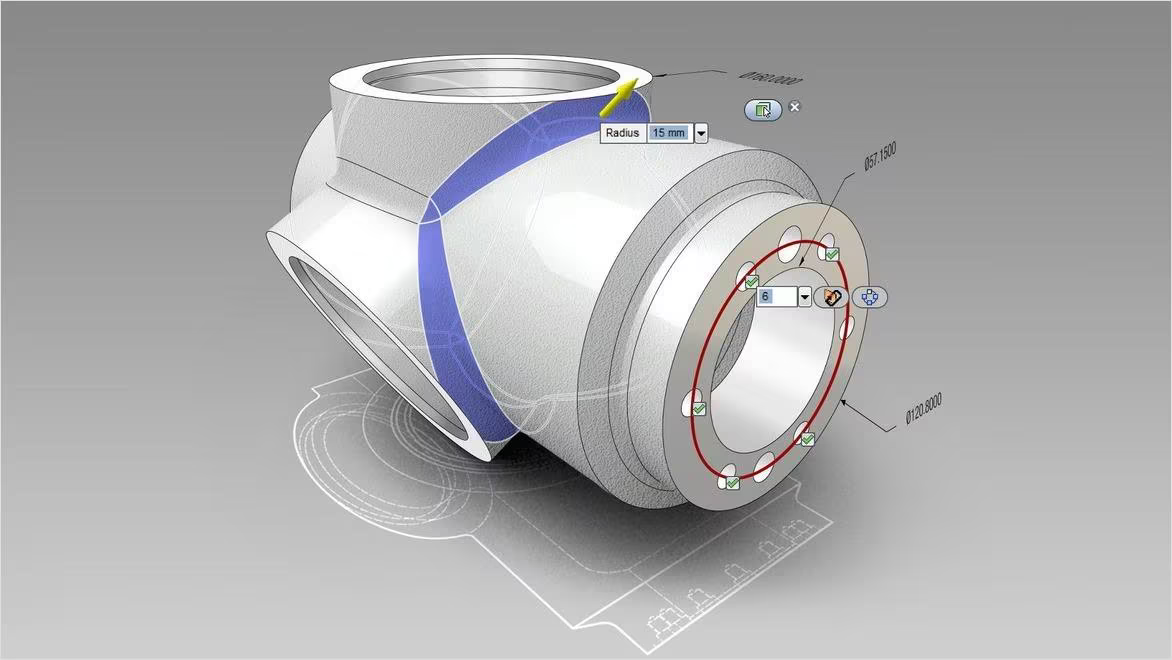
\includegraphics[scale=0.4]{Page2.png}}
		\end{center}
	\end{frame}
	
	%------------------- Quarta slide --------------------
	\begin{frame}{\textbf{Perché ora?}}
		\begin{tabularx}{\linewidth}{XX}
		{
			\begin{center}
					\zoombox{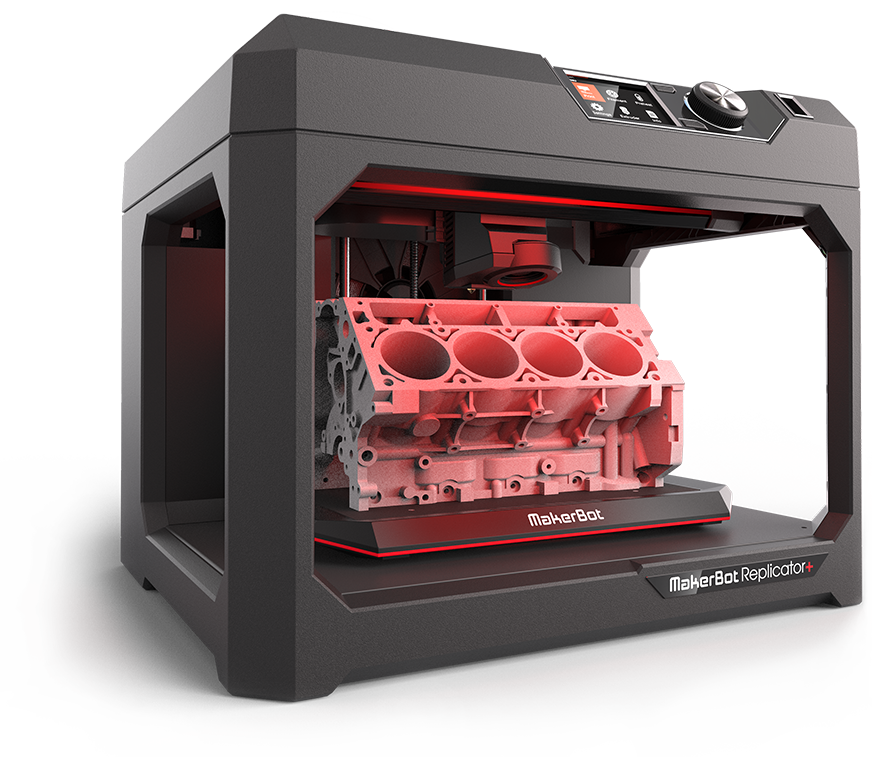
\includegraphics[scale=0.2]{Page3.png}}
			\end{center}
		}&{
			\begin{center}
				\begin{itemize}
					\item I programmi di modellazione 3-D hanno raggiunto una espressività tale da permettere facilmente di modellare ogni tipo di pezzo.
					\item Le stampanti in 3-D sono diventante sempre più economiche e avanzate.
				\end{itemize}
			\end{center}
		}		
		\end{tabularx}
	\end{frame}
	
	%------------------- Quinta slide --------------------
	\begin{frame}{\textbf{Potenzialità di mercato}}
		\begin{tabularx}{\linewidth}{XX}
			{
				\begin{center}
					\vspace*{8mm}
					\zoombox{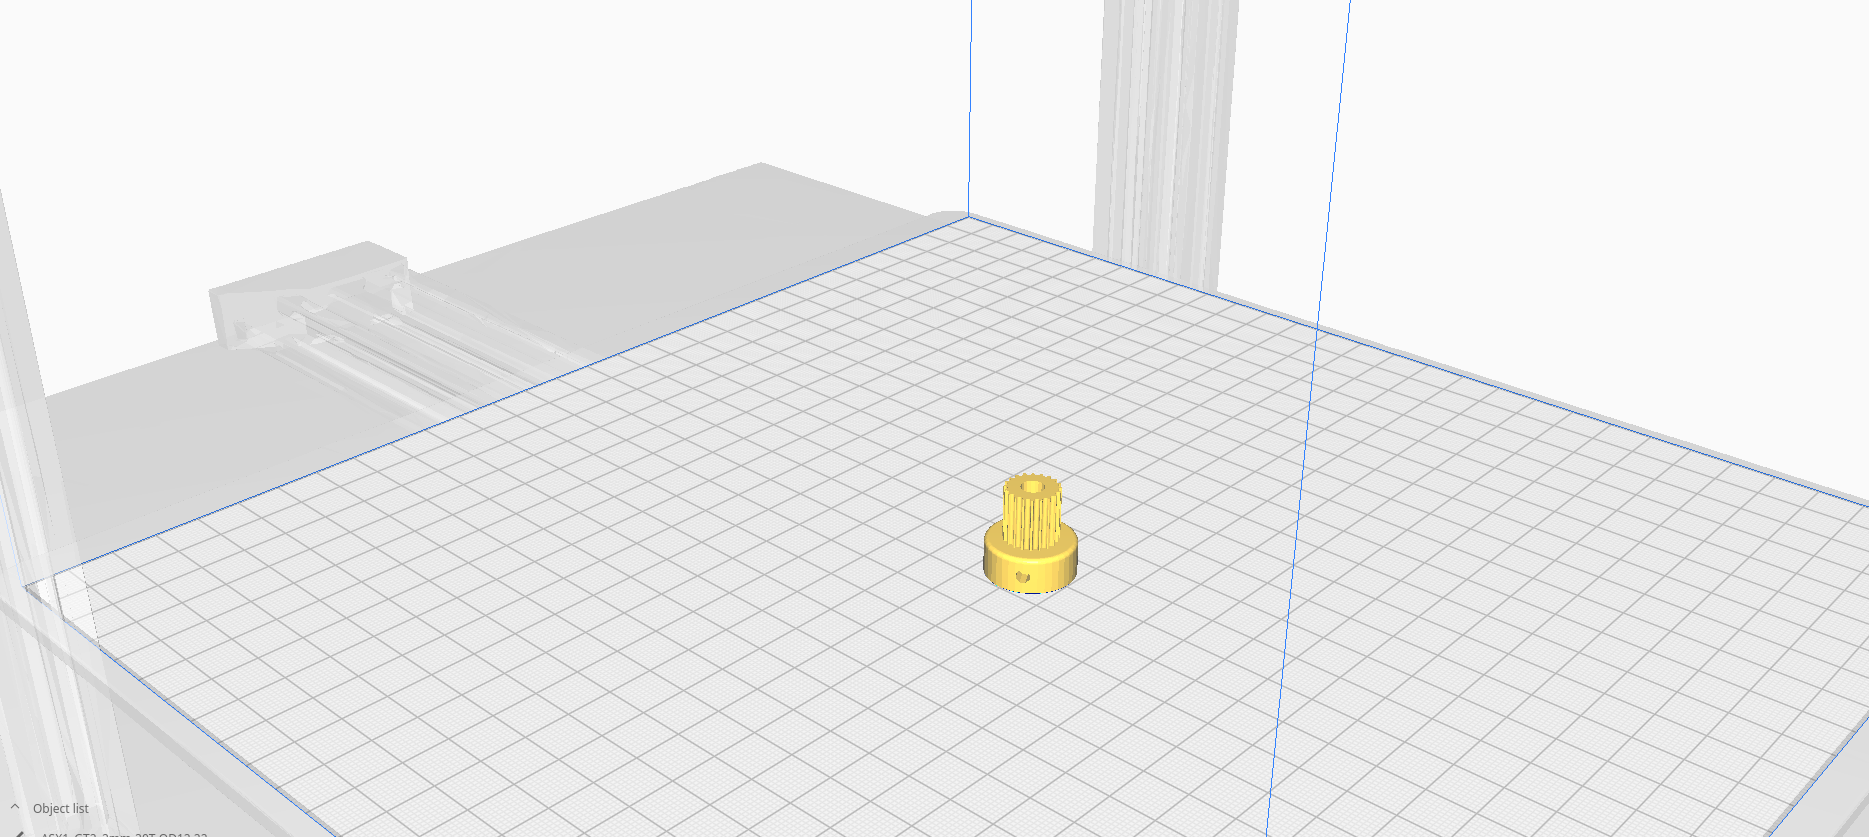
\includegraphics[scale=0.15]{Page4.png}}
				\end{center}
			}&{
				\begin{center}
					\vspace*{15mm}
					\small
					\begin{itemize}
						\item Costo di modellazione prototipo: €25.
						\item Usura meccanica:  produzione costante.
						\item Produzione di 50 unità: €8 al pezzo.
					\end{itemize}
				\end{center}
			}
		\end{tabularx}
	\end{frame}
	
	%------------------- Sesta slide --------------------
	\begin{frame}{\textbf{I concorrenti}}
		\begin{tabularx}{\linewidth}{XX}
			{
				\begin{center}
					\vspace*{15mm}
					\begin{itemize}
						\item Oggi non è più necessario riprodurre le parti di ricambio a mano come una volta facevano gli artigiani.
					\end{itemize}
				\end{center}	
			}&{
				\begin{center}
					\zoombox{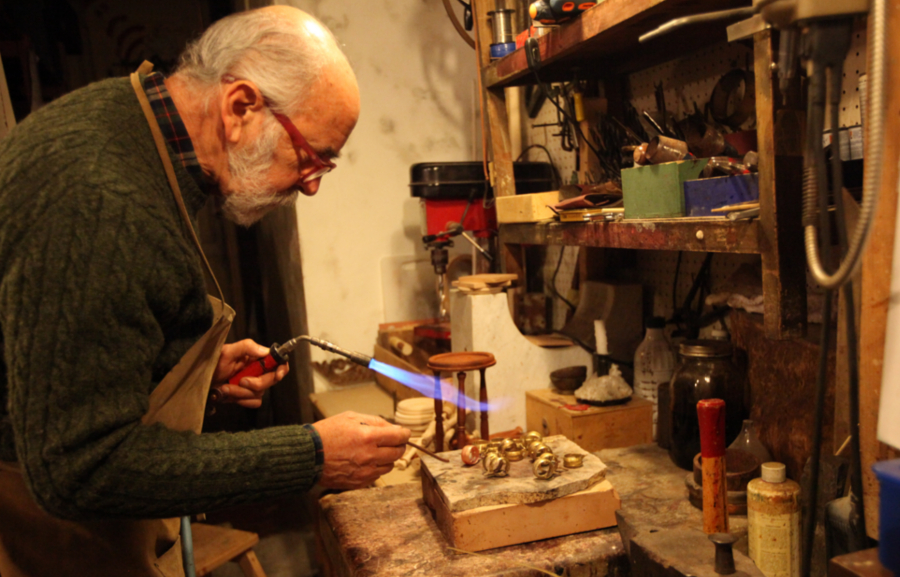
\includegraphics[scale=0.3]{Page5.png}}
				\end{center}
			}
		\end{tabularx}
	\end{frame}

		%------------------- Settima slide --------------------
	\begin{frame}{\textbf{Il business model}}
		\begin{tabularx}{\linewidth}{XX}
			{
			\begin{center}
				\vspace*{16mm}
				\small
				\begin{itemize}
					\item Primo canale di vendita: centri di assistenza di elettrodomestici - Solo a Pesaro 3.
					\item Secondo canale di vendita: centri di assistenza per cantieristica navale - Solo a Pesaro 5.
				\end{itemize}
			\end{center}
			}&{
				\begin{center}
					\zoombox{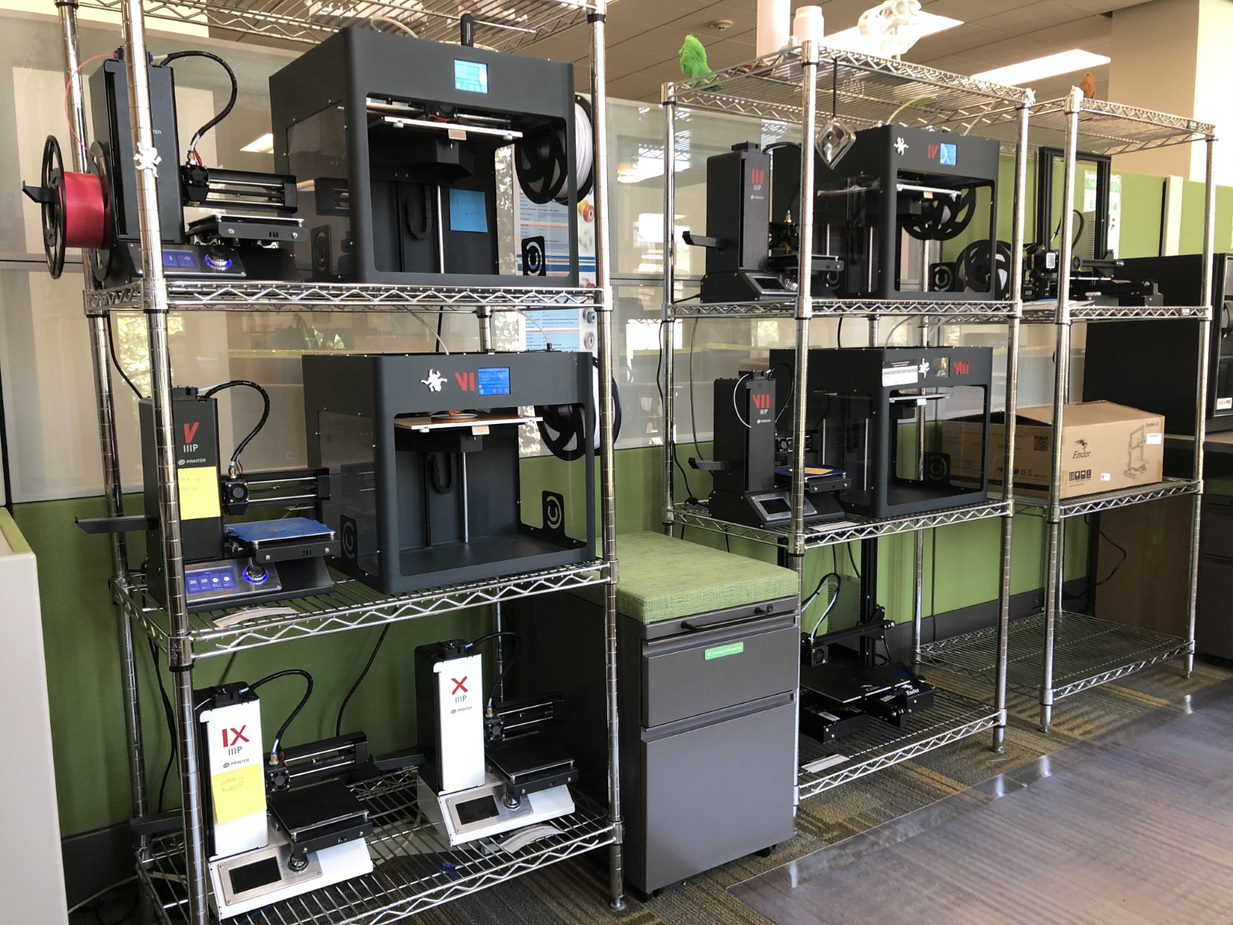
\includegraphics[scale=0.22]{Page6.png}}
				\end{center}
			}
		\end{tabularx}
	\end{frame}
	
	%------------------- Ottava slide --------------------
	\begin{frame}{\textbf{Il team}}
		\begin{center}
			\zoombox{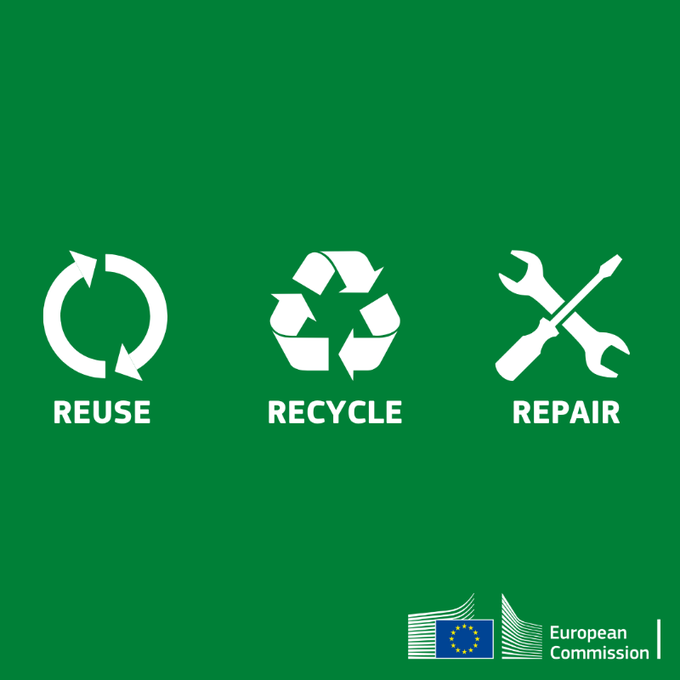
\includegraphics[scale=0.7]{Page7.png}}
		\end{center}
		\begin{tabularx}{\linewidth}{XXX}
			{
			\begin{itemize}
				\item \textbf{Francesco Rombaldoni} \newline
				Informatica applicata \newline
				Esperienza di 2 anni nel settore 3-D
			\end{itemize}
			}&{
			\begin{itemize}
				\item \textbf{Rocco Luigi Ciarfaglia}\newline
				Scienze motorie, sportive e della salute.
			\end{itemize}
			}&{
			\begin{itemize}
				\item \textbf{Marco Belletti}\newline
				Scienze umanistiche.
			\end{itemize}
			}
		\end{tabularx}
	\end{frame}

	%------------------- Nona slide --------------------
	\begin{frame}{\textbf{Quello che ci serve}}
		\begin{tabularx}{\linewidth}{XX}
			{
				\begin{center}
					\vspace*{7mm}
					\begin{itemize}
						\item Conoscere tutti i centri di assistenza del territorio per continuare a vendere il nostro servizio. 
					\end{itemize}
				\end{center}	
			}&{
				\begin{center}
					\zoombox{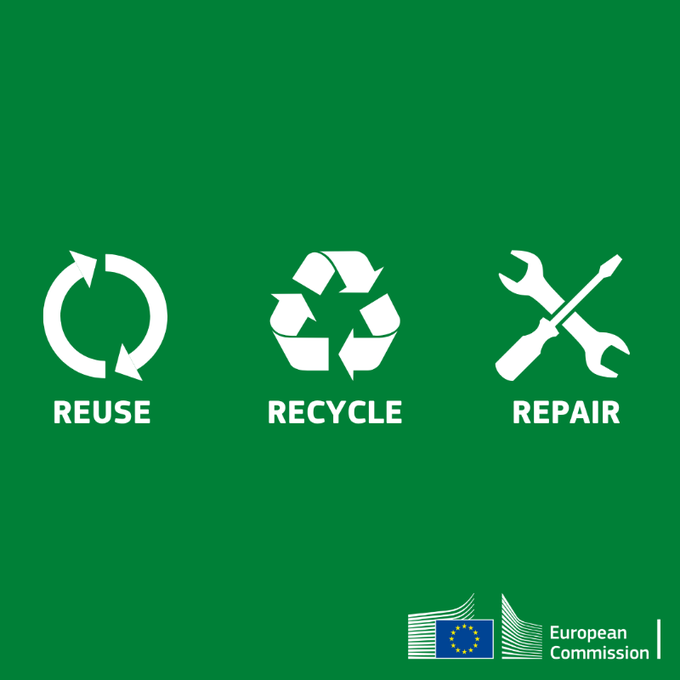
\includegraphics[scale=0.2]{Page8.png}}
				\end{center}
			}
		\end{tabularx}
	\end{frame}
	
	%------------------- Chiusura --------------------

\begin{frame}[plain]
	\maketitle
	\vspace*{5mm}
	\begin{tabularx}{\linewidth}{XX}
		{
			\begin{center}
				\vspace*{-20mm}
				\zoombox{\includegraphics[scale=0.2]{logo_bianco.png}}
			\end{center}
		}&{
			\begin{center}
				\vspace*{-11mm}
				\large
				\textbf{Francesco Rombaldoni}\newline\newline
				\href{f.rombaldoni@campus.uniurb.it}{\textcolor{blue}{f.rombaldoni@campus.uniurb.it}}
			\end{center}
		}
	\end{tabularx}
\end{frame}	
	
	% Frame con la licenza
	\begin{frame}
		\vspace*{\fill}
		% Print license shield
		\doclicenseThis
	\end{frame}
	
\end{document}